\chapter{Experimental Results}
\label{resuls}
%\pagenumbering{arabic} 
In this chapter, we will evaluate:
\begin{itemize}
	\item Different IDT descriptors for the single view action recognition
	\item Cross-view action recognition results with/without transfer learning
	\item Cross-view action recognition results with joint dictionary and transfer learning
\end{itemize}
Detailed results and model parameters analysis will be found in the following sections.

\section{Comparison of Different Descriptors}

Different IDT descriptors are compared to check the performance of each individual descriptor (i.e., HOG, HOF, MBH, TRA) and their combination of all descriptors for each view. The results of MBH are the combination of MBHx, and MBHy channel.\ 
The results in Table~\ref{table1} show that IDT descriptor performance is better than other descriptors for the single view recognition, so this motivates us to apply IDT descriptor for later action recognition experiments.
\begin{table}[h]
	\small
	%\large
	\centering
	\caption{Comparison of IDT descriptors on single view classification.} 
	%\resizebox{\textwidth}{!} {%
	\begin{tabular}{@{\extracolsep{12pt}}llcccc}
		\toprule   
		Data & HOF & HOG & MBH & TRA & IDT\\ 
		\hline
		\midrule
		View1  & 94.25\% & 93.10\% & 95.40\% & 81.60\% & 93.10\%\\
		View2  & 96.55\% & 89.65\% & 64.58\% & 77.61\% & 100\%\\
		View3  & 93.10\% & 93.10\% & 94.20\% & 80.06\% & 97.70\%\\
		\bottomrule
		\hline
		\midrule
	\end{tabular}%
	%	}
	\label{table1}
\end{table}

\section{Cross-View Action Recognition without TL}

To conduct ablation study and show the effectiveness of our joint modeling, first, cross-view action recognition is carried out without using any transfer learning method. The model is trained on Fisher Vector encoded video descriptors after applying dimension reduction with PCA. Basically, the model is trained on one view and tested on another view. In the meanwhile, the single view recognition result is also shown to compare the cross-view results. The results are shown in Table~\ref{table3}. We can see that the single view accuracy (on the diagonal) is between 95\% and 100\% while the cross-view accuracy for different cross-view settings are between 40\% and 55\%, which is much more challenging.
\begin{table}[!ht]
	\centering
	\caption{Cross-view action recognition without TL.} 
	%	\resizebox{\textwidth}{!} {%
	\begin{tabular}{@{\extracolsep{40pt}}cccc}
		\toprule   
		{} &   \multicolumn{3}{c}{Training Data}  \\
		\cmidrule{2-4} 
		Testing Data  & View1 & View2 & View3  \\ 
		\hline
		\midrule
		View1  & 96\% & 44.93\% & 45.26\%  \\ 
		View2  & 41.93\% & 100\% & 48.87\%  \\ 
		View3  & 45.55\% & 52.82\% & 98.85\%  \\ 
		\bottomrule
		\hline
		\midrule
	\end{tabular}%
	%	}
	\label{table3}
\end{table}

\section{Cross-View Action Recognition by TL Methods.}

In this section, different transfer learning methods are applied for cross-view settings, and compared with results without using the transfer learning method under the same setting. The evaluation is done using the four state-of-the-art methods, i.e., TCA, TJM, JDA, and BDA, and their details can be found from the methodology section. 

\noindent
\textbf{Parameters Setting}. Note we do not apply PCA for dimension reduction as all transfer learning methods implement dimension reduction by themselves. For all methods $\lambda$ is set to 1, $\gamma$ is set to 0.1 as given in~\cite{6751384}, and number of dimensions are set to 400. The iteration number is set to 5 due to its performance for all methods except TCA since it is not an iterative process. The BDA requires $\mu$ value which is set to 0 as it provided by default in their package and the linear kernel SVM is used for all methods. 

Results for cross-view action recognition using different transfer learning methods are listed in Table~\ref{table2}. From the table, we can see JDA renders higher accuracy in comparison to all other methods, while TJM results are close to JDA results for cross-view action recognition from View2 to View3 and the results for TCA and BDA are between 45\% and 60\%. This indicates that Transfer Learning methods are performing better as compared to the normal approach without knowledge transfer.
\begin{table}[h]
	\centering
	\caption{Cross-view action recognition by TL methods.} 
	%	\resizebox{\textwidth}{!} {%
	\begin{tabular}{@{\extracolsep{40pt}}cccccc}
		\toprule   
		Source & Target & TCA & TJM & JDA & BDA\\ 
		\hline
		\midrule
		View1  & View2 & 47.04\% & 56.22\% & 71.53\% & 53.22\%\\
		View2  & View1 & 59.47\% & 72.81\% & 71.82\% & 59.37\%\\
		View1  & View3 & 62.18\% & 64.58\% & 69.83\% & 42.92\%\\
		View3  & View1 & 47.38\% & 63.09\% & 72.39\% & 45.92\%\\
		View2  & View3 & 52.97\% & 71.67\% & 72\% & 49.43\%\\
     	View3  & View2 & 55\% & 74.96\% & 75.67\% & 57.99\%\\		
		\bottomrule
		\hline
		\midrule
	\end{tabular}%
	%}
	\label{table2}
\end{table}


\section{Cross-View Action Recognition by DL Method}

In this section, cross-view action recognition is carried out on the dictionary learning features. The model is trained on Fisher Vector encoded video descriptors after applying PCA. The model is trained on one view and tested on another view and the single view recognition result is also shown. The results given in Table~\ref{table3:DL} demonstrate that the single view accuracy is between 95\% and 100\% while cross-view accuracies are between 40\% and 55\%.
\begin{table}[!ht]
	\centering
	\caption{Cross-view action recognition by DL.} 
	%	\resizebox{\textwidth}{!} {%
	\begin{tabular}{@{\extracolsep{40pt}}cccc}
		\toprule   
		{} &   \multicolumn{3}{c}{Training Data}  \\
		\cmidrule{2-4} 
		Testing Data  & View1 & View2 & View3  \\ 
		\hline
		\midrule
		View1  & 85.05\% & 42.18\% & 34.13\%  \\ 
		View2  & 42.18\% & 94.25\% & 49.08\%  \\ 
		View3  & 42.03\% & 45.06\% & 91.95\%  \\ 
		\bottomrule
		\hline
		\midrule
	\end{tabular}%
	%	}
	\label{table3:DL}
\end{table}
%Our method approach
\section{Cross-View Action Recognition by JDTL}
% Highlighted Values\
In this section, we will evaluate our proposed joint learning approach for cross-view action recognition where the model is trained on one view and tested on another view. Table~\ref{table4:topnovel} summarizes the highest accuracy achieved by our novel approach using different cross-view settings and different transfer learning methods. From the table, we can see that TCA is performing well, as accuracy is greater than 90\% for all cross-view combinations. The highest accuracy we got using JDA is 92\%, while BDA and TJM accuracy is between 85\% and 95\%. 


\begin{table}[!ht]
	\centering
	\caption{Cross-view action recognition by JDTL.} 
	%	\resizebox{0.9\textwidth}{2cm} {%
	\begin{tabular}{@{\extracolsep{20pt}}cccccc}
		\toprule   
		Training Data & Testing Data &  TCA & JDA & BDA & TJM\\ 
		\hline
		\midrule
		View1&  View2	& 92.8\%  & 92.01\% &	94.51\%	 &91.77\%\\
		View1&	View3	& 94.02\%  &	89.98\%	&	93.38\%	&	83.84\%\\
		View2&	View1	& 91.34\% &	91.50\%	&	92.48\%	&	90.69\%\\
		View2&  View3	& 96.61\% &	92.41\%	&	90.47\%	&	92.89\%\\
		View3&	View1	& 91.83\% &	88.56\%	&	92.32\%	&	88.24\%\\
		View3&	View2	& 90.32\% &	86.94\%	&	88.55\%	&	85.65\%\\
		\bottomrule
		\hline
		\midrule
	\end{tabular}%
	%	}
	\label{table4:topnovel}
\end{table}
%\noindent
Next, we will lead detailed discussions on three different cross-view settings. As our method works in an iterative way to optimize the features, we are allowed to observe the accuracy change in each iteration for different transfer learning methods. The following sections also discuss the confusion matrix where we are allowed for further diagnosis for our cross-view model.

\subsection{Cross-View Action Recognition by JDTL on View1 and View2}

Table~\ref{table5} and Figure~\ref{fig1:View1-View2} show the results of cross-view action recognition by training the model on View1 and testing on View2 using our novel proposed approach. Table~\ref{table8} and Figure~\ref{fig1:View2-View1} show the results of cross-view action recognition by training on View2 and testing on View1. From these cross-view settings, we can see that BDA and JDA (supervised learning mode) performance is increasing in each iteration and BDA also handles class imbalance. TCA performance in the first six iterations is increasing, but after that there is a small decrease in accuracy of each iteration.%\\

\begin{table}[hbt!]
	\centering
	\caption{Cross-view action recognition by JDTL trained on View1 and tested on View2.} 
	%	\resizebox{0.9\textwidth}{3cm} {%
	\begin{tabular}{@{\extracolsep{12pt}}ccccc}
		\toprule 
		Iteration No. &  TCA & JDA & BDA & TJM\\ 
		\hline
		\midrule
		1 &79.83\%	& 69.03\% &	82.41\%	 &85.16\%\\
		2&	92.25\%	&	73.38\%	&	90.32\%	&	91.77\%\\
		3&	90.8\%	&	70.48\%	&	88.38\%	&	85.8\%\\
		4&	89.67\%	&	80.96\%	&	92.58\%	&	79.51\%\\
		5&	93.54\%	&	87.74\%	&	94.03\%	&	75.84\%\\
		6&	92.25\%	&	90.32\%	&	92.51\%	&	78.81\%\\
		7&	90.96\%	&	90.01\%	&	94.51\%	&	81.77\%\\
		8&	87.74\%	&	92.01\%	&	92.1\%	&	84.7\%\\
		9&	88.06\%	&	91.93\%	&	91.61\%	&	82.6\%\\
		10&	86.45\%	&	91.61\%	&	92.1\%	&	87.41\%\\
		\bottomrule
		\hline
		\midrule
	\end{tabular}%
%	}
	\label{table5}
\end{table}
%\noindent
Confusion matrices are illustrated in Figure~\ref{fig:CMV1V2} and~\ref{fig:CMV2V1} to identify which actions cause confusion with other actions.
Each column represents the ground truth, while each row represents the predicted results.
As seen from Figure~\ref{fig:CMV1V2}, our model presents appealing results using different transfer learning methods for most action classes in cross-view action recognition such as \enquote{Brushing Teeth}, \enquote{Check Time} and \enquote{Cheer Up}. The accuracy of JDA and BDA is relatively worse, because for most of the cases, one of the action classes are not recognized properly, e.g., \enquote{Bow}.
\begin{figure}[hbt!]
		\centering
	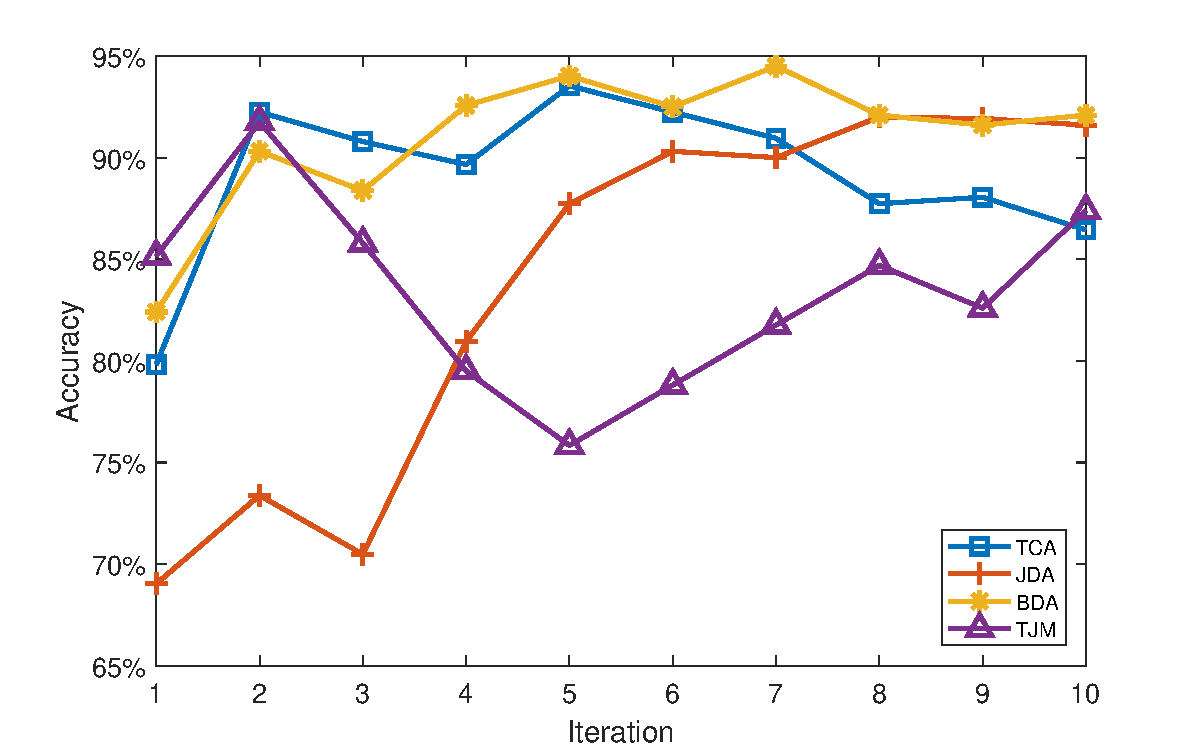
\includegraphics[width=5in,height=3.5in]{figures/plots/View1-View2-2}
	\linebreak
	\caption{Cross-view action recognition by JDTL trained on View1 and tested on View2.}
	\label{fig1:View1-View2}
\end{figure}
%\noindent
Figure~\ref{fig:CMV2V1} shows the confusion matrices when the model is trained on View2 and tested on View1. All classes are properly classified in BDA except \enquote{Brushing Teeth} which is mostly confused with \enquote{Bow} action. The \enquote{Bow} action is creating confusion for other transfer learning methods, such as in TCA, it is confused with \enquote{Cheer Up} action, while in JDA and TJM, it is recognized as \enquote{Brushing Hair}.
%View2-VIew1
\begin{figure}[]
	\centering
	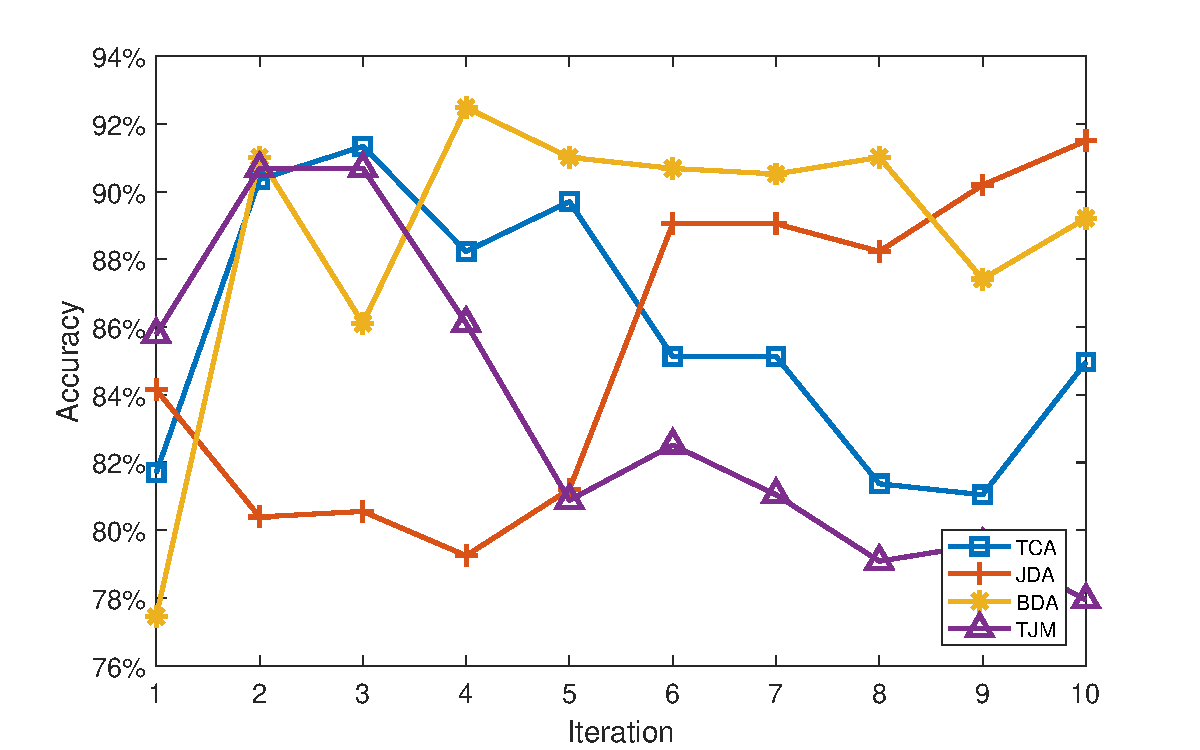
\includegraphics[width=5in,height=3.5in]{figures/plots/View2-View1}
	\linebreak
	\caption{Cross-view action recognition by JDTL trained on View2 and tested on View1.}
	\label{fig1:View2-View1}
\end{figure}

\begin{table}[]
	\centering
	\caption{Cross-view action recognition by JDTL trained on View2 and tested on View1.} 
	%	\resizebox{0.95\textwidth}{3cm} {%
	\begin{tabular}{@{\extracolsep{12pt}}ccccc}
		\toprule   
		Iteration No. &  TCA & JDA & BDA & TJM\\ 
		\hline
		\midrule
		1&	81.70\%&	84.15\%&	77.45\%&	85.78\%\\
		2&	90.36\%&	80.39\%&	91.01\%&	90.69\%\\
		3&	91.34\%&	80.56\%&	86.11\%&	90.69\%\\
		4&	88.24\%&	79.25\%&	92.48\%&	86.11\%\\
		5&	89.71\%&	81.21\%&	91.01\%&	80.88\%\\
		6&	85.13\%&	89.05\%&	90.69\%&	82.52\%\\
		7&	85.13\%&	89.05\%&	90.52\%&	81.05\%\\
		8&	81.37\%&	88.24\%&	91.01\%&	79.08\%\\
		9&	81.05\%&	90.20\%&	87.42\%&	79.58\%\\
		10&	84.97\%&	91.50\%&	89.22\%&	77.94\%\\
		\bottomrule
		\hline
		\midrule
	\end{tabular}%
	%		}
	\label{table8}
\end{table}


\begin{figure}[H]
	\begin{subfigure}{.5\textwidth}
		\centering
		\includegraphics[width=1\linewidth]{"figures/Confusion matrix/BDA/View1View2/V1V2BDA".png}
		\caption{BDA}
		\label{fig:V1V2BDA}
	\end{subfigure}%
	\begin{subfigure}{.5\textwidth}
		\centering
		\includegraphics[width=1\linewidth]{"figures/Confusion matrix/TCA/View1View2/V1V2TCA".png}
		\caption{TCA}
		\label{fig:V1V2TCA}
	\end{subfigure}
	\begin{subfigure}{.5\textwidth}
		\centering
		\includegraphics[width=1\linewidth]{"figures/Confusion matrix/JDA/View1View2/V1V2JDA".png}
		\caption{JDA}
		\label{fig:V1V2JDA}
	\end{subfigure}%
	\begin{subfigure}{.5\textwidth}
		\centering
		\includegraphics[width=1\linewidth]{"figures/Confusion matrix/TJM/View1View2/V1V2TJM".png}
		\caption{TJM}
		\label{fig:V1V2TJM}
	\end{subfigure}
	\caption{Confusion matrix trained on View1 and tested on View2}
	\label{fig:CMV1V2}
\end{figure}



\begin{figure}[H]
	\begin{subfigure}{.5\textwidth}
		\centering
		\includegraphics[width=1\linewidth]{"figures/Confusion matrix/BDA/View2View1/V2V1BDA".png}
		\caption{BDA}
		\label{fig:V2V1BDA}
	\end{subfigure}%
	\begin{subfigure}{.5\textwidth}
		\centering
		\includegraphics[width=1\linewidth]{"figures/Confusion matrix/TCA/View2View1/V2V1TCA".png}
		\caption{TCA}
		\label{fig:V2V1TCA}
	\end{subfigure}
	\begin{subfigure}{.5\textwidth}
		\centering
		\includegraphics[width=1\linewidth]{"figures/Confusion matrix/JDA/View2View1/V2V1JDA".png}
		\caption{JDA}
		\label{fig:V2V1JDA}
	\end{subfigure}%
	\begin{subfigure}{.5\textwidth}
		\centering
		\includegraphics[width=1\linewidth]{"figures/Confusion matrix/TJM/View2View1/V2V1TJM".png}
		\caption{TJM}
		\label{fig:V2V1TJM}
	\end{subfigure}
	\caption{Confusion matrix trained on View2 and tested on View1.}
	\label{fig:CMV2V1}
\end{figure}


\subsection{Cross-View Action Recognition by JDTL on View1 and View3}

Here, we trained the model on View1 and tested on View3 and vice versa. Table~\ref	{table5} and Figure~\ref{fig1:View1-View3} summarize the results for View1 to View3 while Table~\ref{table8} and Figure~\ref{fig1:View3-View1} show the results for View3 to View1. View1 and View3 have mirror videos as those are captured in exact opposite angles. From Figure~\ref{fig1:View1-View3}, we can see that TCA and BDA methods are performing well while JDA and TJM do not have such good results. But in Figure~\ref{fig1:View3-View1}, we can see BDA is performing well as compared to the other methods. The accuracy is increasing for the first five iterations in BDA, and then it is varying with each iteration. In TCA, performance of the first three iteration is increasing, and then it is decreasing with each iteration. The accuracy of JDA and TJM methods does not change too much with each iteration.
\begin{table}[hbt!]
	\centering
	\caption{Cross-view action recognition by JDTL trained on View1 and tested on View3.} 
	%\resizebox{0.7\textwidth}{3cm} {%
		\begin{tabular}{@{\extracolsep{12pt}}ccccc}
			\toprule   
			Iteration No. &  TCA & JDA & BDA & TJM\\ 
			\hline
			\midrule
			1&	86.75\%&	80.29\%&	86.27\%&	70.44\%\\
			2&	90.31\%&	77.38\%&	89.98\%&	67.53\%\\
			3&	91.11\%&	73.02\%&	93.38\%&	67.04\%\\
			4&	92.41\%&	70.60\%&	93.05\%&	69.79\%\\
			5&	94.02\%&	80.45\%&	91.92\%&	72.54\%\\
			6&	91.76\%&	82.07\%&	87.40\%&	73.51\%\\
			7&	93.70\%&	79.97\%&	88.85\%&	78.35\%\\
			8&	92.73\%&	83.52\%&	86.59\%&	77.71\%\\
			9&	92.25\%&	85.62\%&	85.46\%&	83.68\%\\
			10&	93.38\%&	89.98\%&	89.34\%&	83.84\%\\
			\bottomrule
			\hline
			\midrule
		\end{tabular}%
%	}
	\label{table6}
\end{table}

\begin{figure}[hbt!]
	\centering
	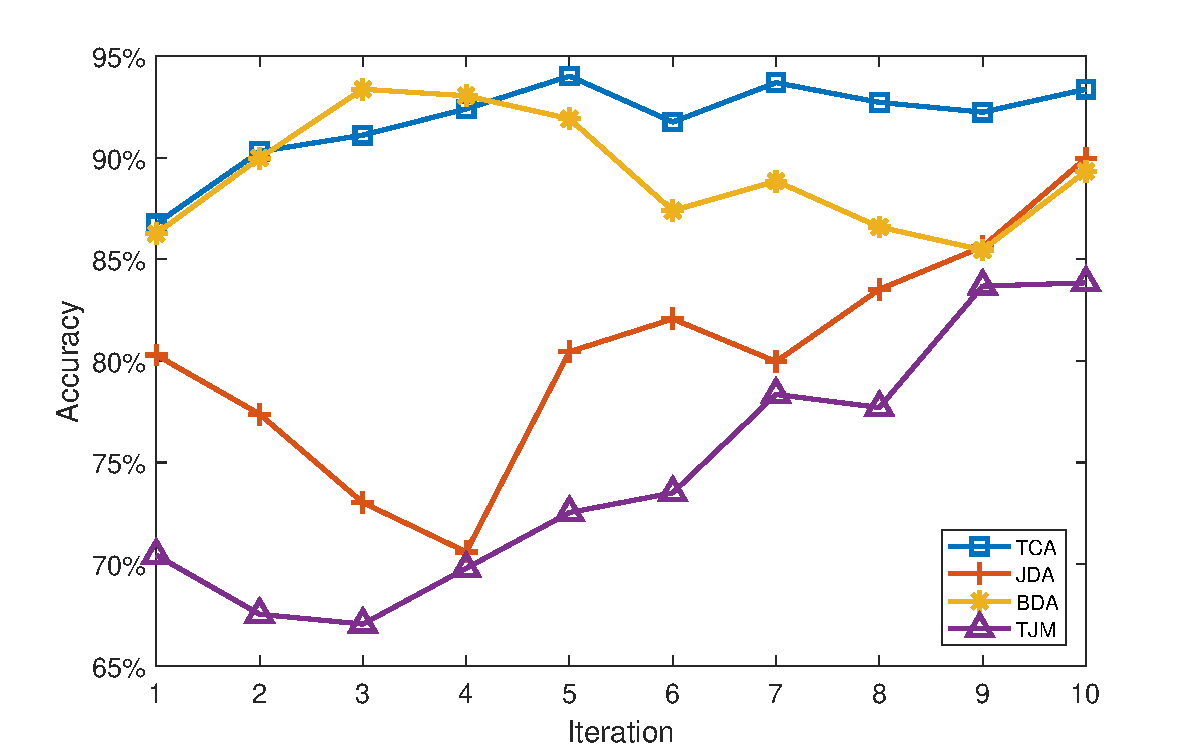
\includegraphics[width=5in,height=3.25in]{figures/plots/View1-View3}
	\linebreak
	\caption{Cross-view action recognition by JDTL trained on View1 and tested on View3.}
	\label{fig1:View1-View3}
\end{figure}


\begin{table}[hbt!]
	\centering
	\caption{Cross-view action recognition by JDTL trained on View3 and tested on View1.} 
	%\resizebox{0.7\textwidth}{3cm} {%
		\begin{tabular}{@{\extracolsep{12pt}}ccccc}
			\toprule
			Iteration No. &  TCA & JDA & BDA & TJM\\ 
			\hline
			\midrule
			1&	70.42\%&	84.31\%&	72.22\%&	79.90\%\\
			2&	87.25\%&	86.93\%&	88.07\%&	84.48\%\\
			3&	91.83\%&	86.93\%&	90.52\%&	86.44\%\\
			4&	87.58\%&	84.31\%&	87.91\%&	86.11\%\\
			5&	85.46\%&	88.56\%&	92.32\%&	85.29\%\\
			6&	85.62\%&	82.35\%&	88.40\%&	85.13\%\\
			7&	84.80\%&	84.31\%&	89.22\%&	85.46\%\\
			8&	84.64\%&	86.60\%&	88.07\%&	86.76\%\\
			9&	84.15\%&	85.95\%&	90.52\%&	88.24\%\\
			10&	83.33\%&	85.29\%&	90.36\%&	86.44\%\\
			\bottomrule
			\hline
			\midrule
		\end{tabular}%
%	}
	\label{table9}
\end{table}


\begin{figure}[hbt!]
	\centering
	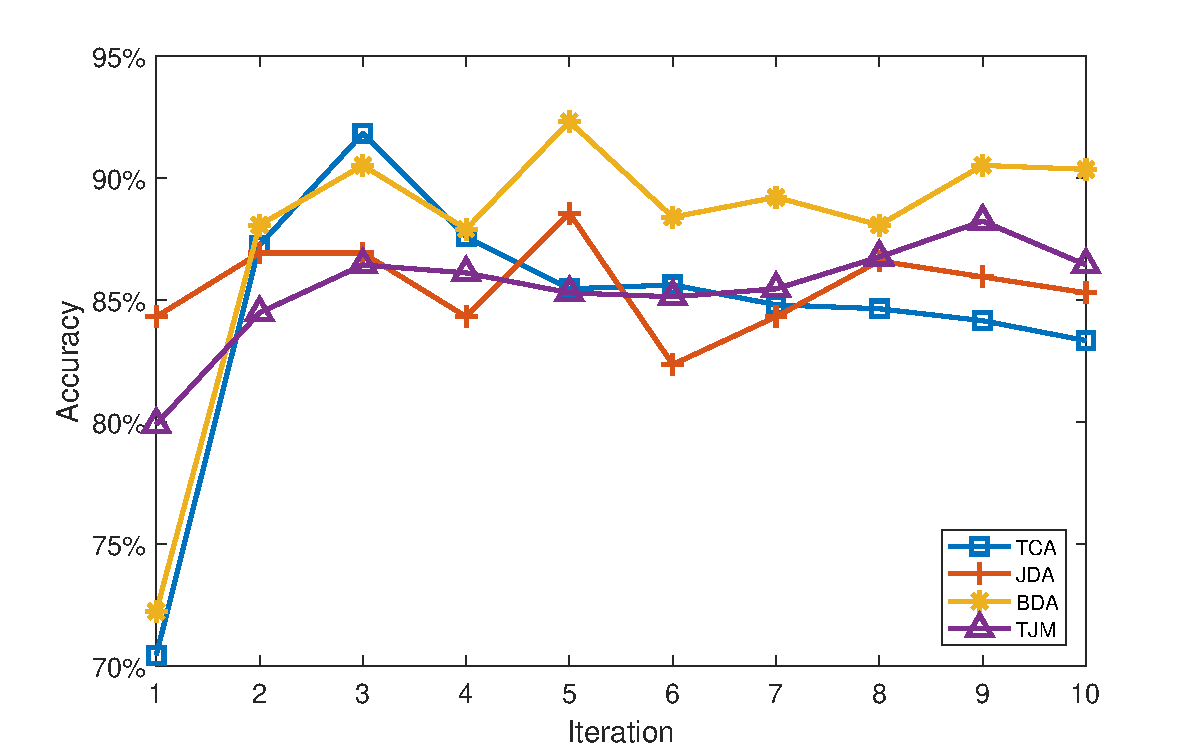
\includegraphics[width=5in,height=3.5in]{figures/plots/View3-View1}
	\linebreak
	\caption{Cross-view action recognition by JDTL trained on View3 and tested on View1.}
	\label{fig1:View3-View1}
\end{figure}

Confusion matrices for these cross-view combinations are given in Figure~\ref{fig:CMV1V3} and Figure~\ref{fig:CMV3V1} for View1 to View3 and View3 to View1, respectively. Figure~\ref{fig:CMV1V3} shows that in BDA and TJM \enquote{Brushing Teeth} is misclassified as \enquote{Check Time} or \enquote{Cheer Up}, while in TCA \enquote{Brushing Hair} and \enquote{Check Time} are mostly confused with each other. From Figure~\ref{fig:CMV3V1}, it can be seen that \enquote{Bow} action is misclassified with all other actions in BDA, JDA and TJM methods, while in JDA and BDA methods \enquote{Cheer Up} action is recognized correctly. In TCA \enquote{Brushing Hair} is misclassified with \enquote{Check Time} and \enquote{Cheer Up} actions.
%% View1 -View 3 table and plot

%% View3- VIew1




\begin{figure}[]
	\begin{subfigure}{.5\textwidth}
		\centering
		\includegraphics[width=1\linewidth]{"figures/Confusion matrix/BDA/View1View3/V1V3BDA".png}
		\caption{BDA}
		\label{fig:V1V3BDA}
	\end{subfigure}%
	\begin{subfigure}{.5\textwidth}
		\centering
		\includegraphics[width=1\linewidth]{"figures/Confusion matrix/TCA/View1View3/V1V3TCA".png}
		\caption{TCA}
		\label{fig:V1V3TCA}
	\end{subfigure}
	\begin{subfigure}{.5\textwidth}
		\centering
		\includegraphics[width=1\linewidth]{"figures/Confusion matrix/JDA/View1View3/V1V3JDA".png}
		\caption{JDA}
		\label{fig:V1V3JDA}
	\end{subfigure}%
	\begin{subfigure}{.5\textwidth}
		\centering
		\includegraphics[width=1\linewidth]{"figures/Confusion matrix/TJM/View1View3/V1V3TJM".png}
		\caption{TJM}
		\label{fig:V1V3TJM}
	\end{subfigure}
	\caption{Confusion matrix trained on View1 and tested on View3}
	\label{fig:CMV1V3}
\end{figure}

\begin{figure}[]
	\begin{subfigure}{.5\textwidth}
		\centering
		\includegraphics[width=1\linewidth]{"figures/Confusion matrix/BDA/View3View1/V3V1BDA".png}
		\caption{BDA}
		\label{fig:V3V1BDA}
	\end{subfigure}%
	\begin{subfigure}{.5\textwidth}
		\centering
		\includegraphics[width=1\linewidth]{"figures/Confusion matrix/TCA/View3View1/V3V1TCA".png}
		\caption{TCA}
		\label{fig:V3V1TCA}
	\end{subfigure}
	\begin{subfigure}{.5\textwidth}
		\centering
		\includegraphics[width=1\linewidth]{"figures/Confusion matrix/JDA/View3View1/V3V1JDA".png}
		\caption{JDA}
		\label{fig:V3V1JDA}
	\end{subfigure}%
	\begin{subfigure}{.5\textwidth}
		\centering
		\includegraphics[width=1\linewidth]{"figures/Confusion matrix/TJM/View3View1/V3V1TJM".png}
		\caption{TJM}
		\label{fig:V3V1TJM}
	\end{subfigure}
	\caption{Confusion matrix trained on View3 and tested on View1.}
	\label{fig:CMV3V1}
\end{figure}

%% View2 -View2 table and plot
%% View2 -View 3 table and plot
\subsection{Cross-View Action Recognition by JDTL on View2 and View3}
Table~\ref{table7} and Figure~\ref{fig1:View2-View3} show the results for cross-view action recognition when the model is trained on View2 and tested on View3 and Table~\ref{table10} and Figure~\ref{fig1:View3-View2} show the results when the model is trained on View3 and tested on View2. We can see in Figure~\ref{fig1:View2-View3}, TCA accuracy is increasing until the seventh iteration and then it is decreasing. In BDA, accuracy increases until sixth iteration and in TJM it increases until fourth iteration. Then performance decreases in both methods. In JDA, accuracy increases until fifth iteration and then it is changing with different iterations.

The Figure~\ref{fig:CMV2V3} shows which action classes are creating confusion when the model is trained on View2 and tested on View3. From the confusion matrices, we can see that \enquote{Bow} action is creating the confusion in BDA, JDA, and TJM transfer learning methods. While in TCA \enquote{Brushing Teeth} is recognized as the \enquote{Cheer Up} or \enquote{Bow} actions.
\begin{figure}[hbt!]
	\centering
	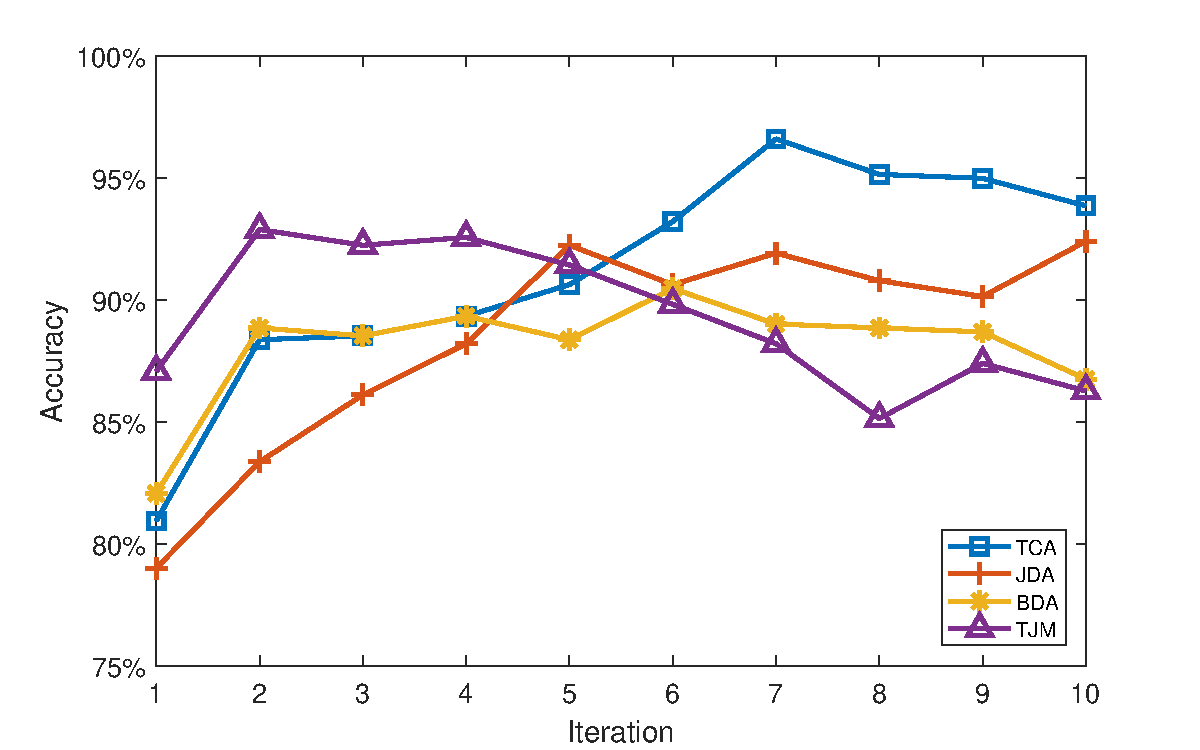
\includegraphics[width=5in,height=3.25in]{figures/plots/View2-View3}
	\linebreak
	\caption{Cross-view action recognition by JDTL trained on View2 and tested on View3.}
	\label{fig1:View2-View3}
\end{figure}

\begin{table}[]
	\centering
	\caption{Cross-view action recognition by JDTL trained on View2 and tested on View3.} 
	%\resizebox{0.7\textwidth}{!} {%
	\begin{tabular}{@{\extracolsep{12pt}}ccccc}
		\toprule   
		Iteration No. &  TCA & JDA & BDA & TJM\\ 
		\hline
		\midrule
		1&	80.94\%&	79.00\%&	82.07\%&	87.08\%\\
		2&	88.37\%&	83.36\%&	88.85\%&	92.89\%\\
		3&	88.53\%&	86.11\%&	88.53\%&	92.25\%\\
		4&	89.34\%&	88.21\%&	89.34\%&	92.57\%\\
		5&	90.63\%&	92.25\%&	88.37\%&	91.44\%\\
		6&	93.21\%&	90.63\%&	90.47\%&	89.82\%\\
		7&	96.61\%&	91.92\%&	89.01\%&	88.21\%\\
		8&	95.15\%&	90.79\%&	88.85\%&	85.14\%\\
		9&	94.99\%&	90.15\%&	88.69\%&	87.40\%\\
		10&	93.86\%&	92.41\%&	86.75\%&	86.27\%\\
		\bottomrule
		\hline
		\midrule
	\end{tabular}%
	%	}
	\label{table7}
\end{table}

%% View3- View2
\begin{figure}[]
	\centering
	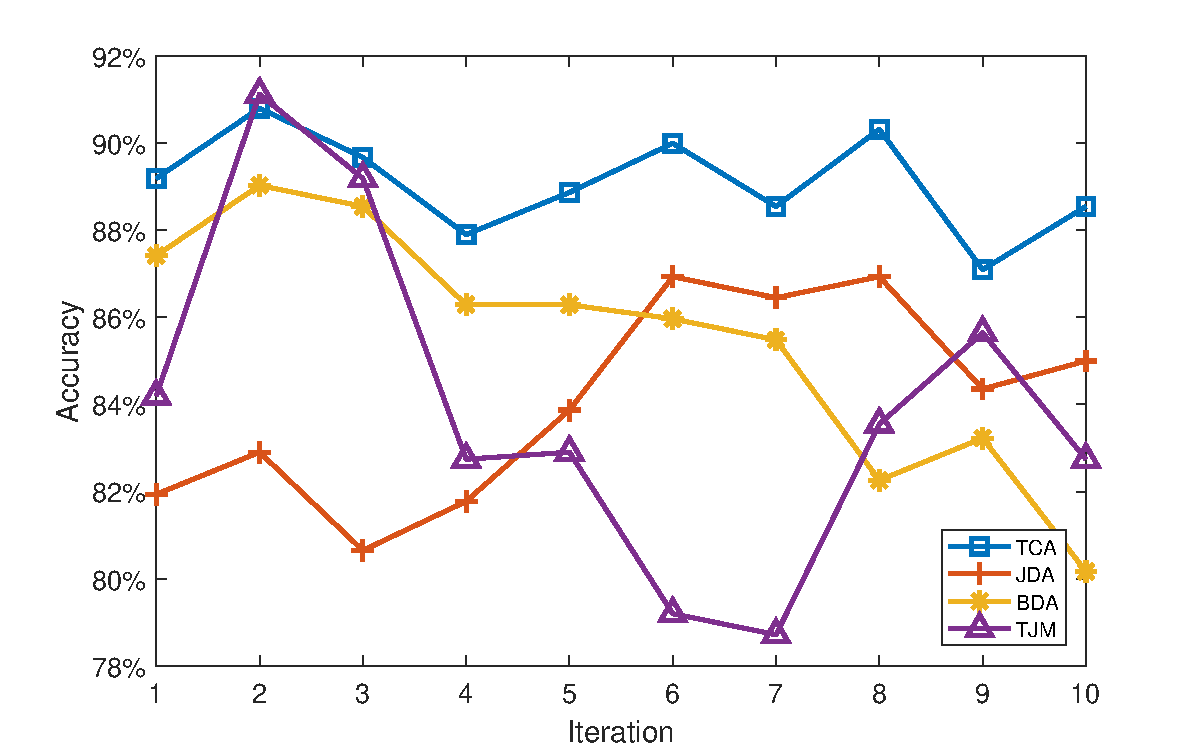
\includegraphics[width=5in,height=3.25in]{figures/plots/View3-View2}
	\linebreak
	\caption{Cross-view action recognition by JDTL trained on View3 and tested on View2.}
	\label{fig1:View3-View2}
\end{figure}

\begin{table}[hbt!]
	
	\centering
	\caption{Cross-view action recognition by JDTL trained on View3 and tested on View2.} 
	%	\resizebox{0.75\textwidth}{!} {%
	\begin{tabular}{@{\extracolsep{12pt}}ccccc}
		\toprule   
		Iteration No. &  TCA & JDA & BDA & TJM\\ 
		\hline
		\midrule
		1&	89.19\%&	81.94\%&	87.42\%&	84.19\%\\
		2&	90.81\%&	82.90\%&	89.03\%&	91.13\%\\
		3&	89.68\%&	80.65\%&	88.55\%&	89.19\%\\
		4&	87.90\%&	81.77\%&	86.29\%&	82.74\%\\
		5&	88.87\%&	83.87\%&	86.29\%&	82.90\%\\
		6&	90.00\%&	86.94\%&	85.97\%&	79.19\%\\
		7&	88.55\%&	86.45\%&	85.48\%&	78.71\%\\
		8&	90.32\%&	86.94\%&	82.26\%&	83.55\%\\
		9&	87.10\%&	84.35\%&	83.23\%&	85.65\%\\
		10&	88.55\%&	85.00\%&	80.16\%&	82.74\%\\
		\bottomrule
		\hline
		\midrule
	\end{tabular}%
	%	}
	\label{table10}
\end{table}

From Figure~\ref{fig1:View3-View2}, we can see that the highest accuracy for TCA, JDA, and TJM is achieved in the second iteration, while in JDA it is achieved in sixth and eighth iteration. As we can see in Figure~\ref{fig1:View3-View2} that JDA accuracy seems to be increasing after third iteration while BDA accuracy is decreasing after second iteration. The accuracy of TCA is stabilized over the iteration while TJM is very unstable. The confusion matrix for this cross-view combination is shown in Figure~\ref{fig:CMV3V2}. \enquote{Bow} and \enquote{Cheer Up} actions are mostly misclassified with different actions in all transfer learning methods. In TCA and BDA \enquote{Cheer Up} and \enquote{Check Time} are misclassified with each other.

\begin{figure}[hbt!]
	\begin{subfigure}{.5\textwidth}
		\centering
		\includegraphics[width=1\linewidth]{"figures/Confusion matrix/BDA/View2View3/V2V3BDA".png}
		\caption{BDA}
		\label{fig:V2V3BDA}
	\end{subfigure}%
	\begin{subfigure}{.5\textwidth}
		\centering
		\includegraphics[width=1\linewidth]{"figures/Confusion matrix/TCA/View2View3/V2V3TCA".png}
		\caption{TCA}
		\label{fig:V2V3TCA}
	\end{subfigure}
	\begin{subfigure}{.5\textwidth}
		\centering
		\includegraphics[width=1\linewidth]{"figures/Confusion matrix/JDA/View2View3/V2V3JDA".png}
		\caption{JDA}
		\label{fig:V2V3JDA}
	\end{subfigure}%
	\begin{subfigure}{.5\textwidth}
		\centering
		\includegraphics[width=1\linewidth]{"figures/Confusion matrix/TJM/View2View3/V2V3TJM".png}
		\caption{TJM}
		\label{fig:V2V3TJM}
	\end{subfigure}
	\caption{Confusion matrix trained on View2 and tested on View3.}
	\label{fig:CMV2V3}
\end{figure}



\begin{figure}[hbt!]
	\begin{subfigure}{.5\textwidth}
		\centering
		\includegraphics[width=1\linewidth]{"figures/Confusion matrix/BDA/View3View2/V3V2BDA".png}
		\caption{BDA}
		\label{fig:V3V2BDA}
	\end{subfigure}%
	\begin{subfigure}{.5\textwidth}
		\centering
		\includegraphics[width=1\linewidth]{"figures/Confusion matrix/TCA/View3View2/V3V2TCA".png}
		\caption{TCA}
		\label{fig:V3V2TCA}
	\end{subfigure}
	\begin{subfigure}{.5\textwidth}
		\centering
		\includegraphics[width=1\linewidth]{"figures/Confusion matrix/JDA/View3View2/V3V2JDA".png}
		\caption{JDA}
		\label{fig:V3V2JDA}
	\end{subfigure}%
	\begin{subfigure}{.5\textwidth}
		\centering
		\includegraphics[width=1\linewidth]{"figures/Confusion matrix/TJM/View3View2/V3V2TJM".png}
		\caption{TJM}
		\label{fig:V3V2TJM}
	\end{subfigure}
	\caption{Confusion matrix trained on View3 and tested on View2.}
	\label{fig:CMV3V2}
\end{figure}
%\noindent 


\section{Discussion}
From the experimental results, it can be concluded that we obtained significant results from different cross-view settings by training the model on one view and recognizing the same action from different views using our joint dictionary and transfer learning method (JDTL). The effectiveness of our proposed approach has been demonstrated by comparing our models with those trained with, or without transfer learning and dictionary learning methods.

As we have discussed earlier that our method works in an iterative manner, the accuracy of most of the transfer learning methods is increasing until fifth iteration. After that, the performance becomes different, which may be caused by the confusion between two actions. For example, from the confusion matrices, we can learn that mostly \enquote{Bow} action is confused with \enquote{Brushing Hair} action.

The JDTL method is efficient as compared to other cross-view or multi-view action recognition methods because in other methods common feature representation is extracted by constructing a connection or mapping between both views. To that end, videos need to be aligned well based on the frame-to-frame, video-to-video, or codebook-to-codebook criteria. In our method, however, we did not construct any mapping, as dictionary learning is used to extract discriminative features and transfer learning is used to project those discriminative features into common subspace, which provides better time and memory efficacy.

In this study, we evaluated our method on the action classes with only a single person performing some actions in a closed and fixed environment. It will become more complex but attractive in recognizing actions of an individual person when multiple people exist and act differently. This will reflect most real-world scenarios for action recognition. Also, in our study, we considered five action classes for the evaluations, while we may further explore other classes to testify the robustness of our model, and its real-world values.


